%
% inverse.tex -- slide template
%
% (c) 2021 Prof Dr Andreas Müller, OST Ostschweizer Fachhochschule
%
\bgroup
\begin{frame}[t]
\setlength{\abovedisplayskip}{5pt}
\setlength{\belowdisplayskip}{5pt}
\frametitle{Involution/Inverse}
\vspace{-20pt}
\begin{columns}[t,onlytextwidth]
\begin{column}{0.48\textwidth}
\begin{center}
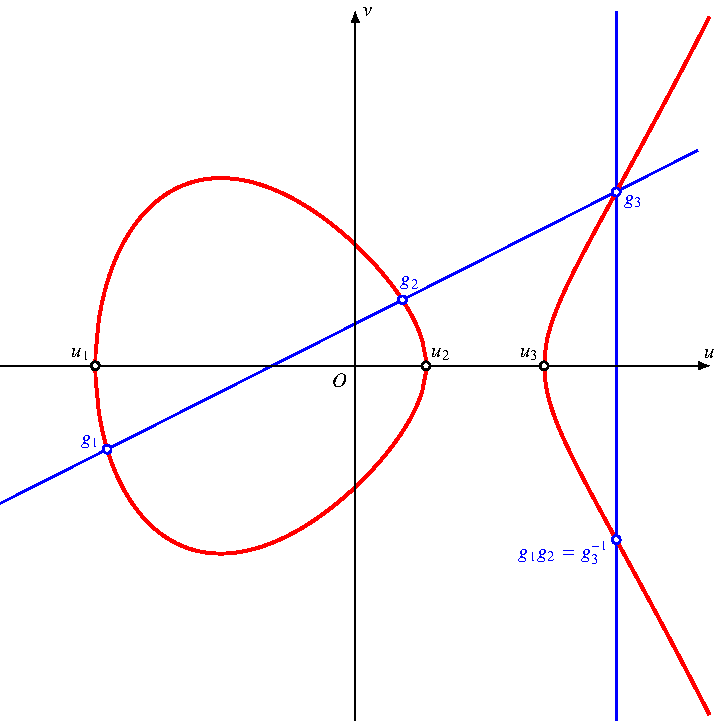
\includegraphics[width=\textwidth]{../../buch/chapters/90-crypto/images/elliptic.pdf}
\end{center}
\end{column}
\begin{column}{0.48\textwidth}
\begin{block}{In speziellen Koordinaten}
\vspace{-12pt}
\[
v^2 = u^3+Au+B
\]
\uncover<2->{invariant unter $v\mapsto -v$}%
\\
\uncover<3->{{\color{red}geht nicht in $\mathbb{F}_2$}}
\end{block}
\uncover<4->{%
\begin{block}{Allgemein}
\vspace{-12pt}
\begin{align*}
Y^2+XY &= X^3 + aX+b
\\
\uncover<5->{%
Y(Y+X) &= X^3 + aX + b}
\end{align*}
\uncover<6->{invariant unter}
\begin{align*}
\uncover<7->{X&\mapsto X,& Y&\mapsto -X-Y}
\\
\uncover<8->{&&\Rightarrow X+Y&\mapsto -Y}
\end{align*}
\uncover<9->{Spezialfall $\mathbb{F}_2$: $Y\leftrightarrow X+Y$}
\end{block}}
\end{column}
\end{columns}
\end{frame}
\egroup
